A central concept in signal processing is that a signal can be expressed as a linear superposition of sinusoids.\footnote{More generally, functions can be thought of as vectors and expressed as linear superpositions of basis vectors, where the basis is chosen to suit the problem at hand. In problems with translation invariance, sinusoids are convenient because they are eigenvectors of translation. For example, defining $E: \reals \rightarrow \complexes$ by the equation $E(t) = \exp(i \omega t)$, we have $E(t + \delta t) = \exp(i \omega \delta t) E(t)$.}
The usual Fourier transform expresses a function $f: \reals \rightarrow \complexes$ as a continuous superposition i.e. integral
\begin{equation}
  f(t) = \int \frac{d \omega}{2\pi} \tilde{f}(\omega) e^{i \omega t} \, .
\end{equation}
The utility and properties of the Fourier transform should be at least somewhat familiar to the audience of this book; if not, see ??.
However, the Fourier transform pertains to function defined over a domain of infinite extent and with infinite resolution.
In real life applications with e.g. experimental data, discrete time digital devices such as digital-to-analog converters (DAC) and analog-to-digital (ADC) converters, or in crystals with discrete unit cells, we have either finite domains, finite resolution, or both.
What we imagine to be less familar to readers here, is how to handle the subtleties introduced in those cases.

As suggested above, there are four major Fourier transforms, each characterized by the extent of its domain and the resolution on that domain.
These transforms are listed in Table~\ref{tab:four_transforms}.
\begin{table}
  \begin{center}
    \begin{tabular}{|r|c|c|c|c|}
      \hline
      \textbf{Name}                   & \textbf{Extent}  & \textbf{Resolution}  & \textbf{Transformed extent}   & \textbf{Transformed resolution} \\
      \hline
      \hline
      Fourier transform               & infinite                & continuous                  & infinite                & continuous \\
      \hline
      Discrete time Fourier transform & infinite                & discrete                    & finite                  & continuous \\
      \hline
      Fourier series                  & finite                  & continuous                  & infinite                & discrete \\
      \hline
      Discrete Fourier transform      & finite                  & discrete                    & finite                  & discrete \\
      \hline
    \end{tabular}
    \caption{The four Fourier transforms}
    \label{tab:four_transforms}
  \end{center}
\end{table}
Let's go through the cases in table one at time.
To clarify the language, we talk about functions (i.e. signals) of time whose transforms are functions of frequency.
However these considerations apply to functions defined over space, or anything else.
As illustrated above, the Fourier transform (FT) maps a continous function over the full real line to another continous function over the full real line.
That is, given an infinite extent of time with infinite time resolution, we have a transform defined over infinite extent of frequency with infinite frequency resolution.

\leveldown{Discrete time Fourier transform (DTFT)}
Suppose that our function is defined over the integers, i.e. the time samples run infinitely far into the past and future, but with discrete instead of continous resolution $\delta t$.
Intuitively, this function cannot have frequency components with frequencies beyond $1/\delta t$, so we should expect the transformed function to be defined only within a finite range $[0, 1/\delta t]$.
This is the case with the discrete time Fourier transform (DTFT), which maps a function $f: \integers \rightarrow \complexes$ defined on the integers to a function $F: [0, 1] \rightarrow \complexes$ defined on a finite but continuous interval:
\begin{equation}
  f_n = \int_0^1 d\nu \, F (\nu) e^{i 2 \pi \nu n}
  \qquad
  F(\nu) = \sum_{n=-\infty}^\infty f_n e^{-i 2\pi \nu n}
  \, .
\end{equation}
Compared to the Fourier transform, the DTFT has limited frequency extent because the original signal is not known with enough time resolution to resolve frequencies beyond $1/\delta t$.

\levelstay{Fourier series (FS)}
Suppose that our function is defined over a continous but finite interval $[0, T]$, i.e. the time runs over a limited range but with infinite resolution.
Intuitively, this function cannot have frequency components distinguished more finely than $1/T$, so we should expect the transformed function to be defined over a discrete set of frequencies separated by $\delta f = 1 / T$.
This is the case with the Fourier series (FS), which maps a function $f: [0, 1] \rightarrow \complexes$ defined over a finite continous interval to a function $F: \integers \rightarrow \complexes$ defined over the integers:
\begin{equation}
  f(t) = \sum_{k=-\infty}^\infty F_k e^{i 2 \pi t k}
  \qquad
  F_k = \int dt \, f(t) e^{-i 2 \pi t k}
  \, .
\end{equation}
Compared to the Fourier transform, the FS has limited frequency resolution because the original signal is not known for long enough time to resolve the difference between two frequencies closer together than $\delta f = 1 / T$.
Notice that the DTFT and FS are opposites.

\levelstay{Discrete Fourier transform (DFT)}
Now suppose that our function is defined over a finite set of discrete samples $\{0, \delta t, 2 \delta t,\ldots, T = (N-1) \delta t\}$.
In this case, we have the limitations of both the DTFT and the FS, i.e. we expect our transformed function to be defined only up to a maximum frequency $1 / \delta t$ and only with frequency resolution $\delta f = 1 / T$.
This is the case with the discrete Fourier transform (DFT), which maps a function $f: \{0, 1,\ldots N-1\} \rightarrow \complexes$ to a function $\tilde f: \{0, 1,\ldots N-1\}$:
\begin{equation}
  f_n = \sum_{k=0}^{N-1} \tilde{f}_k e^{i 2 \pi n k}
  \qquad
  \tilde{f}_k = \sum_{n=0}^{N-1} f_n e^{-i 2 \pi n k}
  \, .
\end{equation}
Compared to the Fourier transform, the DFT has both limited freuqency range and limited frequency resolution.

\levelstay{Outline}

In the remainder of this chapter, we investigate the consequences of the finite and infinite time resolution and extent of these transforms.


\levelstay{Driving} \label{sec:driving}

\leveldown{Capacitive driving}

We next consider driving signals applied to the circuit.
We attach a driving voltage source to our parallel LC through a capacitor $C_d$, as shown by the dotted elements in Fig.\,\ref{Fig:singleCircuit}.
The capacitor $C_d$ is required to prevent the driving circuit from completely ruining the coherence of the main circuit.
Without the capacitor, the loaded quality factor $Q_d$ of the main circuit due to the drive circuit would be \citeinternalref{loadedMode}
\begin{equation}
Q_d = R_d / Z_{LC} .
\end{equation}
With typical circuit impedances in the range 10's to 100's of Ohms, and RF source resistances of $50\,\Omega$\,\footnote{Commercial RF devices essentially \emph{all} use 50 \, $\Omega$ output impedance. This is simply due to the fact that a coaxial transmission line of reasonable size has near $50 \, \Omega$ impedance. The impedance depends logarithmically on geometric parameters and so cannot be significantly varied. 50$ \, \Omega$ has been chosen as a common standard.}, we have $Q_d \approx 1$ which is far too low to be useful in a quantum device.\footnote{The energy relaxation time of the circuit is $T_1 = Q_d / \omega$, so for a 1 GHz device $Q_l=1$ corresponds to $T_1=0.16 \, \text{ns}$.}

The coupling capacitor $C_d$ helps preserve the circuit coherence.
If $C_d$ is sufficiently small, its impedance $Z_{C_d} = 1/i\omega C_d$ is large and the current flowing through $R_d$ is reduced.
Therefore, $C_d$ prevents the process by which energy from the oscillator gets into $R_d$ and is lost.
To be specific, in the limit $Z_{C_d} \gg R_d$ the loaded quality factor of the oscillator is \citeinternalref{loadedMode}
\begin{equation}
Q_l = \left( \frac{C}{C_d} \right)^2 \frac{Z_{LC}}{R_d} .
\end{equation}
Therefore, a small $C_d$ preserves the circuit's coherence.
However, decoupling the drive line from the driving voltage source with a small $C_d$ also limits the speed with which we can control the circuit, so a balance must be struck.
This balance is discussed in full quantitative detail later.

Let's now turn back to formal analysis of the driven circuit, starting with a qualitative prediction.
The main capacitor $C$ is shunted by the series combination of the coupling capacitor $C_d$, and the resistor $R_d$.
Because  $Z_{C_d} \gg R_d$ the impedance of the driving circuit is dominated by $C_d$ which simply adds in parallel with $C$.
Therefore, we expect the effective capacitance of the mode to be $C+C_d$.

Denoting the time dependent driving voltage by $V_d(t)$ and ignoring for now the resistance of the source, we work out Kirchhoff's equation of motion for the driven system, resulting in
\begin{equation}
\frac{1}{1+C/C_d} \dot{V}_d = \ddot{\Phi} + \frac{\omega_0^2}{1 + C_d/C} \Phi. \end{equation}
This is totally sensible: the drive strength increases as $C_d$ increases, and the resonance frequency of the LC mode has shifted due to the new capacitance.
This equation of motion is produced by the Lagrangian
\begin{equation}
\mathcal{L} = \frac{1}{2}C \dot{\Phi}^2 - \frac{1}{2L}\Phi^2 + \frac{1}{2} C_d \left( \dot{\Phi} - V_d \right)^2 \, .
\end{equation}
For the sake of identifying canonical coordinates we consider the case $V_d=0$, resulting in canonical variables
\begin{equation*}
  \Phi
  \qquad \textrm{and} \qquad
  \frac{\partial \mathcal{L}}{\partial \dot{\Phi}} = \left( C + C_d \right) \dot{\Phi} \equiv Q
\end{equation*}
just as before, except that now the capacitance associated to the momentum $Q$ is $C+C_d$ instead of just $C$, which makes sense because $C_d$ is in parallel with $C$.
The Hamiltonian is
\begin{equation}
  H = \frac{Q^2}{2 (C + C_d)} + \frac{\Phi^2}{2L} \, .
\end{equation}
Now we consider what happens when the drive turns on.
The term added to the Lagrangian by the drive is
\begin{equation}
  \mathcal{L}_d = \frac{1}{2}C_d V_d(t)^2 - C_d \dot{\Phi} V_d(t) \, .
\end{equation}
The first term is of no consequence as it does not involve the dynamical variables.
The second term couples the drive to the momentum $Q$, resulting in a Hamiltonian term
\begin{equation*}
H_d
  = C_d \dot{\Phi}V_d(t)
  = \frac{1}{1+C/C_d} Q V_d(t) \, . \label{eq:sec:driving:H_dVsCircuitParams}
\end{equation*}
Now suppose the drive is on resonance with one particular transition $\ket{n} \rightarrow \ket{n+1}$ and far off resonance from any other transition.
In this case we can restrict the analysis to just the states involved in the driven transition.\footnote{The restriction to two levels whose transition is on resonance with the drive is properly justified in the rotating frame, discussed later.}
Because the wave functions of a one-dimensional quantum Hamiltonian are real and because $Q = -i \hbar d/d\Phi$, we can write
\begin{equation*}
  \bbraket{n}{Q}{n+1} = -i \abs{\bbraket{n}{Q}{n+1}} \, ,
\end{equation*}
and using that we can write $H_d$ as
\begin{align*}
  H_d
  &= \frac{V_d(t)}{1 + C / C_d}
    \left[ \begin{array}{cc}
      \bbraket{n}{Q}{n} & \bbraket{n}{Q}{n+1} \\
      \bbraket{n+1}{Q}{n} & \bbraket{n+1}{Q}{n+1}
    \end{array}\right] \\
  &= \frac{V_d(t)}{1 + C / C_d} \left(
      \frac{S_Q}{2} \mathbb{I}
    + \frac{\Delta_Q}{2} \sigma_z
    + \abs{\bbraket{n}{Q}{n+1}} \sigma_y
  \right)
\end{align*}
where $S_Q \equiv \bbraket{n}{Q}{n} + \bbraket{n+1}{Q}{n+1}$ and $\Delta_Q \equiv \bbraket{n}{Q}{n} - \bbraket{n+1}{Q}{n+1}$.
Going back to our definition of the $a$ operator, we can rewrite $Q$ as
\begin{equation*}
  Q = -i Q_\text{zpf} (a - a^\dagger)
\end{equation*}
and if the system is approximately harmonic, then $\bbraket{n}{Q}{n} \approx 0$, $\bbraket{n+1}{Q}{n+1} \approx 0$, and $\bbraket{n}{Q}{n+1} \approx Q_\text{zpf} \sqrt{n+1}$, so
\begin{equation*}
  H_d = \frac{V_d(t)}{1 + C / C_d} \sqrt{n+1} \, Q_\text{zpf} \, \sigma_y
  \, .
\end{equation*}
Later, we will express this driving Hamiltonian in the rotating frame of the qubit.
However, we can already see one important point: the coupling of the drive signal to the circuit scales with the zero point fluctuations in the circuit's charge, and therefore inversely with $\sqrt{Z_{LC}}$.
In other words, low impedance would appear to give stronger coupling.
However, one must be careful about what is being held constant.
Assuming fixed $\omega_{LC}$ and $C \gg C_d$, we find that the drive Hamiltonian is proportional to
\begin{equation}
  \omega_{LC} \sqrt{Z_{LC}}
\end{equation}
which increases for \emph{increasing} impedance.
These same arguments apply to qubit-qubit coupling, as will be described below.

\textbf{Summary - Simple derivation:} The energy stored in the drive capacitor is $E_d = \frac{1}{2}C_d\left( V_d - V_q \right)^2$.
Keeping only the terms involving both the qubit and drive voltages yields \begin{equation}
E_d = - C_d V_d V_q = - C_d V_d \frac{Q}{C} \end{equation}
where $Q$ is the qubit charge.
This matches the full result up to the sign, in the practical limit $C \gg C_d$.


\levelstay{Inductive driving}

\begin{figure}
\begin{centering}
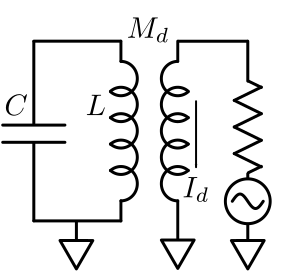
\includegraphics[width=5cm]{inductive_drive.pdf}
\par\end{centering}
  \caption{Parallel LC driving through a mutual inductance.}
\label{fig:qubits.inductive_drive}
\end{figure}

We now consider the case in which we drive by applying current into an inductor which is coupled to the qubit inductor through a mutual inductance $M_d$, as shown in Figure \ref{fig:qubits.inductive_drive}.
With a drive current $I_d(t)$ Kirchhoff's law for the circuit yields the equation of motion
\begin{equation}
  \ddot{\Phi} + \omega_{LC}^2 \Phi = I_d \, \omega_{LC}^2 M_d \, .
\end{equation}
This equation is reproduced by the Lagrangian
\begin{equation}
  \mathcal{L} = \frac{1}{2}C \dot{\Phi}^2 - \frac{1}{2L} \Phi^2 + \frac{M_d}{L}I_d(t) \Phi \, .
\end{equation}
The momentum conjugate to $\Phi$ is
\begin{equation}
  \frac{\partial \mathcal{L}}{\partial \dot{\Phi}} = C \dot{\Phi} = Q
\end{equation}
and the Hamiltonian is
\begin{equation}
  H
  = Q \dot{\Phi} - \mathcal{L}
  = \frac{Q^2}{2C} + \frac{\Phi^2}{2L} - \frac{M_d}{L} I_d(t) \Phi
\end{equation}
so the driving Hamiltonian is
\begin{equation}
  H_d = - \frac{M_d}{L}I_d(t) \Phi \, .
\end{equation}
Note that adding a parallel junction to the circuit does \emph{not} change the form of $H_d$; the junction adds a term $(I_c \Phi_0 / 2\pi)\cos(\pi \Phi / \Phi_0)$ to the Lagrangian, but this term does not couple to $I_d$.
Just as we did for the capacitive drive, we can express the restriction of the inductive drive Hamiltonian two a two-level subspace as
\begin{equation*}
  H_d = -\frac{M_d}{L} I_d(t) \left(
      \frac{S_\Phi}{2} \mathbb{I}
    + \frac{\Delta_\Phi}{2} \sigma_z
    + \abs{\bbraket{n}{\Phi}{n+1}} \sigma_x
  \right)
\end{equation*}
where $S_\Phi = \bbraket{n}{\Phi}{n} + \bbraket{n+1}{\Phi}{n+1}$ and $\Delta_\Phi = \bbraket{n}{\Phi}{n} - \bbraket{n+1}{\Phi}{n+1}$.
Just as in the capacitive case, we can rewrite $\Phi$ in terms of the raising and lowering operators
\begin{equation*}
  \Phi = \Phi_\text{zpf} (a + a^\dagger)
\end{equation*}
and if the system is approximately harmonic then
\begin{equation*}
  H_d = - \frac{M_d}{L} I_d(t) \sqrt{n+1} \, \Phi_\text{zpf} \, \sigma_x
  \, .
\end{equation*}


\section{Coupling}

\subsection{Capacitive coupling}

\begin{figure}
\begin{centering}
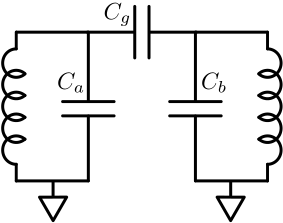
\includegraphics[width=6cm]{coupled_circuits_capacitive.pdf}
\par\end{centering}
\caption{Two circuits coupled through a capacitor $C_g$.}
\label{Fig:coupledCircuits_capacitive}
\end{figure}

The circuit shown in Fig.\,\ref{Fig:coupledCircuits_capacitive} has the following Lagrangian \begin{align}
\mathcal{L} = & \frac{1}{2}C_1\dot{\Phi}_1^2 + \frac{1}{2}C_2\dot{\Phi}_2^2 \nonumber \\
& + \frac{1}{2}C_g \left( \dot{\Phi}_1 - \dot{\Phi_2} \right)^2 \nonumber \\
& - \frac{1}{2L_1}\Phi_1^2 - \frac{1}{2L_2}\Phi_2^2 \, . \end{align}
The kinetic term can be rewritten as \begin{equation}
T = \frac{1}{2}
\left( \begin{array}{cc} \dot{\Phi}_1 & \dot{\Phi}_2 \end{array} \right)
\left( \begin{array}{cc} C_1' & -C_g \\ -C_g & C_2' \end{array} \right)
\left( \begin{array}{c} \dot{\Phi}_1 \\ \dot{\Phi}_2 \end{array} \right) \label{eq:kineticInFlux} \end{equation}
where $C_1' \equiv C_1+C_g$ and similarly for $C_2'$. The canonical momenta are \begin{eqnarray}
p_1 = \frac{dL}{d\dot{\Phi}_1} = C_1'\dot{\Phi}_1 - C_g\dot{\Phi}_2 \nonumber \\
p_2 = \frac{dL}{d\dot{\Phi}_2} = C_2'\dot{\Phi}_2 - C_g\dot{\Phi}_1 \end{eqnarray}
which can be written as \begin{equation}
\left( \begin{array}{c} p_1 \\ p_2 \end{array} \right) =
\left( \begin{array}{cc} C_1' & -C_g \\ -C_g & C_2' \end{array} \right)
\left( \begin{array}{c} \dot{\Phi}_1 \\ \dot{\Phi}_2 \end{array} \right) \end{equation}
Note the recurrence of the matrix from equation (\ref{eq:kineticInFlux}). Naming this matrix $M$ we can write \begin{eqnarray}
T &=& \frac{1}{2}
      \left( \begin{array}{cc} \dot{\Phi}_1&\dot{\Phi}_2 \end{array} \right)
      M
      \left( \begin{array}{c} \dot{\Phi}_1 \\ \dot{\Phi}_2 \end{array} \right) \label{eq:kineticWithM} \\
\left( \begin{array}{c} \dot{\Phi}_1 \\ \dot{\Phi}_2 \end{array} \right) &=& M^{-1} \left( \begin{array}{c} p_1 \\ p_2 \end{array} \right) \label{eq:fluxToMomenta} \end{eqnarray}
Substituting equation (\ref{eq:fluxToMomenta}) into (\ref{eq:kineticWithM}) and using the facts that matrix transposition commutes with matrix inversion and that $M$ is symmetric we get
\begin{equation}
T = \frac{1}{2} \left( \begin{array}{cc} p_1&p_2 \end{array} \right) M^{-1} \left( \begin{array}{c} p_1 \\ p_2 \end{array} \right) \, .
\end{equation}
The inverse of the 2x2 matrix $M$ is
\begin{align}
M^{-1} &= \frac{1}{C_1C_2 + C_g(C_1 + C_2)} \left( \begin{array}{cc} C_2' & C_g \\ C_g & C_1' \end{array} \right) \nonumber \\
&\equiv \left( \begin{array}{cc} 1/C_1'' & 1/C_g'' \\ 1/C_g'' & 1/C_2'' \end{array} \right) \, .
\end{align}
Finally, the kinetic term of the Langrangian is \begin{equation}
T = \frac{p_1^2}{2C_1''} + \frac{p_2^2}{2C_2''} + \frac{p_1p_2}{C_g''} \, . \label{eq:kineticInP}
\end{equation}

Let us now understand the quantities $C_1''$ and $C_2''$ in a simple way.
The capacitance to ground from the signal node of circuit 1 is \begin{eqnarray}
C_{1,\textrm{total}} &=& C_1||(C_g \textrm{ in series with } C_2) \nonumber \\
&=& C_1 + \frac{C_g C_2}{C_g+C_2} \nonumber \\
&=& \frac{C_1 C_2 + C_g(C_1+C_2)}{C_g+C_2} \nonumber \end{eqnarray}
which is exactly equal to our expression for $C_1''$.
Therefore we've found that \textbf{the effective capacitance associated with the the canonical charge is just the capacitance to ground of the conjugate flux's signal node}.

The quantities $p_1$ and $p_2$ have dimensions of charge so we will rename them $\tilde{Q}_1$ and $\tilde{Q}_2$.
The tildes remind us that they are not the usual single qubit charges.

The coupling term in the Hamiltonian, eq.\,(\ref{eq:kineticInP}), is \begin{equation}
H_g = \frac{ \tilde{Q}_1 \tilde{Q}_2} {C_g''}. \label{eq:sec:coupling:H_g} \end{equation}
We would like to re-express it in terms of Pauli operators.
If we use the (very good) approximation that the normal modes are harmonic we can rewrite the charge operators as \begin{equation}
\tilde{Q} = -i Q_{\textrm{zpf}} (a - a^{\dagger}) \, . \end{equation}
The parameter $Q_{\textrm{zpf}}$ is the rms zero point fluctuations in charge and is given by (see \citeinternaltype \citeinternalref{quantumOscillator}) \begin{equation}
Q_{\textrm{zpf}} = \sqrt{\frac{\hbar}{2Z}} = \sqrt{\frac{\hbar \omega C}{2}} \, . \end{equation}
Substitution of this expression for the $\tilde{Q}$ coordinates turns the coupling Hamiltonian into
\begin{align}
H_g &= \frac{Q_{1,\textrm{zpf}}Q_{2,\textrm{zpf}}}{C_g''}(-i)(a_1-a_1^{\dagger})(-i)(a_2-a_2^{\dagger}) \nonumber \\
&= \frac{\hbar}{2}\sqrt{\omega_1\omega_2 C_1'' C_2''}\frac{C_g}{C_1C_2 + C_g(C_1+C_2)}(\sigma_y \otimes \sigma_y) \nonumber \\
&= \frac{1}{2}\frac{C_g}{\sqrt{C_1' C_2'}} \hbar\sqrt{\omega_1\omega_2} (\sigma_y \otimes \sigma_y) \nonumber
\end{align}
where we have again used a two level approximation \mbox{$a - a^\dagger \rightarrow i \sigma_y$}.
We combine the prefactors into a parameter $g$ and write the Hamiltonian as \begin{equation}
H_g = g \left( \sigma_y \otimes \sigma_y \right) \end{equation}
where $g$, called the ``coupling strength'', is defined as \begin{equation}
g \equiv \frac{1}{2} \frac{C_g}{\sqrt{C_1' C_2'}} \hbar\sqrt{\omega_1\omega_2} \, . \end{equation}
Taking $C_1 \approx C_2$ and $\omega_1 \approx \omega_2$, then using $C = 1 / \omega Z_{LC}$ we find
\begin{equation}
g \propto Z_{LC} \, .
\end{equation}

\subsection{Summary - Simple derivation}

The energy in the coupling capacitor is
\begin{equation}
E_g = \frac{1}{2} C_g \left( V_1 - V_2 \right)^2 \, . \nonumber
\end{equation}
Keeping only the term which couples the qubits, we find \begin{equation}
E_g = -C_g V_1 V_2 = -C_g \frac{Q_1}{C_1} \frac{Q_2}{C_2} . \end{equation}
This matches Eq.\,(\ref{eq:sec:coupling:H_g}), up to the sign, in the practical limit $C_1,C_2 \gg C_g$.

\subsection{Inductive Coupling}

\begin{figure}
\begin{centering}
\includegraphics[width=6cm]{coupled_circuits_inductive.pdf}
\par\end{centering}
\caption{Two circuits coupled through a mutual inductance $M$.}
\label{Fig:coupledCircuits_inductive}
\end{figure}


Consider the circuit shown in Figure \ref{Fig:coupledCircuits_inductive}.
From Kirchoff's laws we find that the equations of motion for the system are
\begin{align}
\omega_1^2 Q_1 &= -\ddot{Q}_1 - \left(M/L_1\right) \ddot{Q}_2 \\
\omega_2^2 Q_2 &= -\ddot{Q}_2 - \left(M/L_2\right) \ddot{Q}_1
\end{align}
These equations of motion can be derived from the following Lagrangian
\begin{equation}
\mathcal{L} = \frac{Q_1^2}{2 C_1} + \frac{Q_2^2}{2 C_2}
- \frac{L_1}{2}\dot{Q}_1^2
- \frac{L_2}{2}\dot{Q}_2^2
- M \dot{Q}_1 \dot{Q}_2 \, . \label{eq:sec.coupling.subsec.inductiveCoupling:Lagrangian}
\end{equation}

In this Lagrangian the charges have appeared as the coordinate variables.
This is annoying because in all of our previous analysis we regarded the fluxes as the coordinates and the charges as the conjugate momenta.
To convert to using flux as the coordinate, we note that the $\dot{Q}$ are the loop currents, and we relate the currents to the fluxes using the definition of inductance and mutual inductance:
\begin{align}
\Phi_1 &= L_1 I_1 + M I_2 \\
\Phi_2 &= M I_1 + L_2 I_2 \, .
\end{align}
These equations are rewritten as a matrix equation
\begin{align}
\left( \begin{array}{c} \Phi_1 \\ \Phi_2 \end{array} \right) &=
\left[ \begin{array}{cc} L_1 & M \\ M & L_2 \end{array} \right]
\left( \begin{array}{c} I_1 \\ I_2 \end{array} \right) \\
\ket{\Phi} &= \mathbf{M} \ket{I} \label{eq:sec.coupling.subsec.inductiveCoupling:fluxToI} \, .
\end{align}
Next, using $\dot{Q}=I$, note that the dotted terms in Eq.\,(\ref{eq:sec.coupling.subsec.inductiveCoupling:Lagrangian}) can also be written as a matrix expression:
\begin{equation}
-\frac{1}{2} \bbraket{I}{\mathbf{M}}{I} \, .
\end{equation}
Therefore, by using Eq.\,(\ref{eq:sec.coupling.subsec.inductiveCoupling:fluxToI}) in Eq.\,(\ref{eq:sec.coupling.subsec.inductiveCoupling:Lagrangian}) we can rewrite the Lagrangian as
\begin{equation}
\mathcal{L} =
\frac{Q_1^2}{2 C_1} + \frac{Q_2^2}{2 C_2}
- \frac{1}{2} \bbraket{\Phi}{\mathbf{M}^{-1}}{\Phi} \, .
\end{equation}
To get a true Lagrangian we have to express the charges in terms of flux.
Using the definition of capacitance, $C = Q/V$, and noting that the \emph{total} flux through each inductor is the time integral of the voltage, we have
\begin{equation}
\frac{1}{2}\frac{Q^2}{C} = \frac{1}{2}C \dot{\Phi}^2 \, .
\end{equation}
Using this and expanding $\mathbf{M}^{-1}$ we finally arrive at
\begin{align}
\mathcal{L} &=
\frac{1}{2}C_1 \dot{\Phi}_1^2 + \frac{1}{2}C_2 \dot{\Phi}_2^2 \\
&- \left( \frac{1}{1 - M^2 / L_1L_2} \right)
\left( \frac{\Phi_1^2}{2L_1} + \frac{\Phi_2^2}{2L_2} \right) \\
&+ \left( \frac{1}{1 - M^2 / L_1 L_2} \right) \frac{M}{L_1 L_2} \Phi_1 \Phi_2 \, .
\end{align}
Thus we have reformulated the Lagrangian with the fluxes as the coordinates.

The conjugate momenta are
\begin{equation}
p = \frac{\partial \mathcal{L}}{\partial \dot{\Phi}} = C \dot{\Phi} = Q \, .
\end{equation}
The Hamiltonian is
\begin{align}
H &= \sum_i Q_i \dot{\Phi}_i - \mathcal{L} \\
&= \frac{Q_1^2}{2 C_1} + \frac{Q_2^2}{2 C_2} \\
&+ \left( \frac{1}{1 - M^2 / L_1L_2} \right)
\left( \frac{\Phi_1^2}{2L_1} + \frac{\Phi_2^2}{2L_2} \right) \\
&+ \left( \frac{1}{1 - M^2 / L_1 L_2} \right) \frac{M}{L_1 L_2} \Phi_1 \Phi_2 \, .
\end{align}


\section{Rotating Frame}

The driving and coupling Hamiltonians we have written down are not well suited for calculations because they do not commute with the intrinsic qubit Hamiltonian, which is typically proportional to either $\sigma_x$ or $\sigma_z$.
This non-commutativity is the mathematical manifestation of the physical fact that, in the lab frame, the qubit state processes about an axis in the Block sphere.
For this reason, it is much easier to reason in a frame that rotates about that axis at a frequency near or equal to the resonance frequency of the device, i.e. in a rotating frame.
In this section we show how to re-express the driving and coupling Hamiltonians in a rotating frame.

The single qubit Hamiltonian for single nearly harmonic qubits like the transmon is \begin{equation}
H_q/\hbar = -\frac{\omega_q}{2}\sigma_z \end{equation}
where $\omega_q = \omega_0 + \delta\omega$. Think of $\omega_0$ as an idle point frequency and $\delta \omega$ as a dynamic detuning.
The Schrodinger picture time evolution operator is $T=\exp \left[-i H/\hbar \right]$.
In order to remove the idle point precession of the qubit state, we take as the rotation operator \begin{equation}
R = T^{\dagger} = \exp \left[ -i \frac{\omega_0}{2} t \sigma_z \right], \end{equation}
eg. we rotate the frame by the idle frequency of the qubit.
We compute the remaining effective Hamiltonian $H'$ according to \citeinternalref{quantumMechanics} \begin{eqnarray}
H'/\hbar &=& i\dot{R}R^{\dagger} + R \frac{H_q}{\hbar} R \\
&=& i \left(-i \frac{\omega_0}{2} \right)\sigma_z RR^{\dagger} + R\frac{H_q}{\hbar}R^{\dagger} \\
&=& -\frac{\delta\omega}{2}\sigma_z. \end{eqnarray}
This is precisely the Hamiltonian of a qubit with frequency $\delta\omega$.
In other words, if we go into a frame rotating at the idle frequency of the qubit, what remains is just the qubit precession at the detuning frequency.
In particular if the frame rotates at the same frequency as the qubit the Hamiltonian becomes zero.

\subsection{Operators}

Since we are going to want to work in a frame in which the qubit intrinsic Hamiltonian is zero it will be useful to find the form of various operators in that frame.
We list here the transformation of the Pauli operators under a frame rotating about the z-axis at frequency $\omega_r$.
The rotation operator is $R=\exp \left[-i \frac{1}{2} \omega_r t \sigma_z \right]$ \citeinternalref{quantumMechanics} and the transformed Pauli operators are \begin{align}
R\sigma_xR^{\dagger} & = \cos(\omega_r t)\sigma_x + \sin(\omega_r t) \sigma_y \nonumber \\
R\sigma_yR^{\dagger} & = \cos(\omega_r t)\sigma_y - \sin(\omega_r t) \sigma_x \nonumber \\
R\sigma_zR^{\dagger} & = \sigma_z \nonumber \\
R\sigma_+R^{\dagger} & = e^{i\omega_r t}\sigma_+ \nonumber \\
R\sigma_-R^{\dagger} & = e^{-i\omega_r t}\sigma_- \, . \nonumber \end{align}

\subsection{Driving}

We now consider the driving Hamiltonian in the rotating frame.
From section \ref{sec:driving} we have the general driving Hamiltonian in the lab frame
\begin{equation}
H_d = h_d f(t) \sigma \, .
\end{equation}
For charge driving, we have $\sigma = \sigma_y$, $V_d(t) = V_d f(t)$, and $h_d = \bbraket{1}{Q}{0} V_d/(1 + C/C_d)$.
For flux driving, we have $\sigma = \sigma_x$, $I_d(t) = I_d f(t)$, and $h_d = (M/L) \bbraket{1}{\Phi}{0} I_d$.
We consider the flux case to for the sake of a specific example.
We use the rotation operator \begin{equation}
R = \exp \left[ -i \frac{\omega_r}{2} t \sigma_z \right] \end{equation}
to find the transformed driving Hamiltonian \begin{align}
RH_d R^{\dagger}/h_d
&= e^{-i \frac{\omega_r}{2} t \sigma_z} f(t)\sigma_x e^{i \frac{\omega_r}{2} t \sigma_z} \nonumber \\
&= f(t)\left[ \cos\left(\omega_r t\right)\sigma_x + \sin\left(\omega_r t\right)\sigma_y \right]. \label{eq:drivingH}
\end{align}
Now suppose $f(t)$ is a sinusoid with an envelope $e(t)$,
\begin{align}
& f(t)
= e(t)\cos \left( \omega_d t + \phi_d \right) \\
&= e(t) \left[ \cos \left( \phi_d \right) \cos \left( \omega_d t \right) - \sin \left( \phi_d \right) \sin \left( \omega_d t \right) \right] \\
&= e(t) \left[ I \cos\left(\omega_d t\right) + Q \sin \left(\omega_d t\right) \right] \label{eq:drivingFunctionIQ}
\end{align}
where $I \equiv \cos(\phi_d)$ and $Q \equiv - \sin(\phi_d)$.
Multiplying everything in Eq. (\ref{eq:drivingH}) together and throwing out the high frequency terms we get
\begin{align}
& RH_dR^{\dagger}/h_d \\
&= \frac{e(t)}{2} \left[ \cos(\delta\omega t + \phi_d)\sigma_x - \sin(\delta\omega t + \phi_d)\sigma_y \right] \\
&= \frac{e(t)}{2} \left[ e^{-i(\delta \omega t + \phi_d)} \sigma_+ + e^{i(\delta \omega t + \phi_d)} \sigma_- \right]
\end{align}
where $\delta\omega \equiv \omega_d - \omega_r$. In matrix form this reads
\begin{equation}
RH_dH^{\dagger}/h_d = \frac{e(t)}{2} \left( \begin{array}{cc} 0 & e^{i(\delta\omega t + \phi_d)} \\ e^{-i(\delta\omega t + \phi_d)} & 0 \end{array}\right) \, . \label{eq:drivingH_matrixForm}
\end{equation}
If the drive is on resonance with the frame, and therefore on resonance with the qubit, then we are left with
\begin{align}
RH_dR^{\dagger}/h_d
&= \frac{e(t)}{2}\left( \begin{array}{cc} 0 & e^{i\phi_d} \\ e^{-i\phi_d} & 0 \end{array}\right) \\
&= \frac{e(t)}{2} \left[ I \sigma_x + Q \sigma_y \right] .
\end{align}
This is a rotation about a time independent axis in the xy plane of the Bloch sphere.
If the rotating frame frequency is the same as the qubit frequency, then the qubit Hamiltonian is zero and our on-resonance drive leads to a purely latitudinal rotation on the Bloch sphere with the angle of the rotation axis in the xy plane given by $\phi$.
If the qubit frequency does not match the rotating frame then the qubit Hamiltonian has a residual $\sigma_z$ component and the the rotation axis will be out of the xy plane.

\subsubsection{$\pi$ pulse}

For a resonant drive with $\phi_d=0$ we have \begin{equation}
RH_dR^{\dagger} = -\frac{e(t)}{2}\frac{V_d \left| \bbraket{1}{Q}{0} \right|} {1 + C/C_d} \sigma_x. \end{equation}
The evolution of the qubit under this drive is given by the unitary operator \begin{equation}
U(t) = \exp \left[ i \left( \frac{1}{2 \hbar} \frac{V_d \left| \bbraket{1}{Q}{0} \right|} {1 + C/C_d} \int dt \, e(t) \right) \sigma_x \right]. \end{equation}
This results in a pi pulse when $U(t)=\sigma_x$. Since \begin{equation}
\exp \left[ i \alpha \sigma_x \right] = \cos(\alpha)\textrm{I} + i \sin(\alpha)\sigma_x \end{equation}
we see that the pi pulse occurs when \begin{equation}
\frac{1}{2\hbar} \frac{V_d \left| \bbraket{1}{Q}{0} \right|} {1 + C/C_d} \int e(t) dt = \frac{\pi}{2} \, . \end{equation}
This relation is used to determine the appropriate drive capacitance $C_d$ when designing a device.
The accessible values of $V_0$ are determined by the dynamic range of available pulse generators, the level of attenuation needed to remove noise from the drive lines.
The value of $C_d$, is then chosen to be large enough that a $\pi$-pulse can be done in an acceptably short time while preserving the qubit coherence as discussed above.
The value of $Q_{\textrm{zpf}}$ is determined by the type of qubit.

\subsubsection{Programming for experiment}

Now that we know what the driving Hamiltonian looks like in the rotating frame we can investigate how to program our IF inputs to the IQ mixer to acheive a rotation on the Bloch sphere.
From \citeinternalref{IQMixer} we know that an input IQ signal $e(t)\exp\left[i\omega t + \phi\right]$ produces an RF signal $ e(t)\cos\left[(\omega_c+\omega)t + \phi \right]$, where $\omega_c$ is the carrier frequency. Using trig identities we can rewrite this RF signal as \begin{equation}
e(t) \left[ I\cos(\left[\omega_c+\omega\right] t) + Q\sin(\left[\omega_c+\omega\right]t)\right] \nonumber \end{equation}
where $I=\cos(\phi)$ and $Q=-\sin(\phi)$.
This exactly matches the form we assumed for $f(t)$ in eq. (\ref{eq:drivingFunctionIQ}) if we take $\omega_c + \omega = \omega_d$.
Therefore if we choose $\omega$ such that $\omega + \omega_c = \omega_q$ and work in the rotating frame of the qubit, the driving Hamiltonian is \begin{equation}
H_d/h_d = \frac{e(t)}{2}\left[I\sigma_x + Q\sigma_y\right]. \end{equation}
In practice we don't want to have to remember to account for the carrier frequency when programming a pulse so we define a mix function which multiplies our complex signal by $\exp\left[i(\omega_{q} - \omega_c)\right]$.
That way if we program a signal $\exp\left[i\phi\right]$ the driving Hamiltonian in the frame of the qubit is produced in the following steps \begin{align}
&\textrm{program} e(t) e^{i\phi} \nonumber \\
&\stackrel{\textrm{mix function}}{\longrightarrow} e(t) e^{i([\omega_q-\omega_c]t + \phi)} \nonumber \\
&\stackrel{\textrm{physical mixer}}{\longrightarrow} \Re \left[ e(t) e^{i(\omega_q t + \phi)} \right] = e(t) \cos\left(\omega_q t + \phi \right) \nonumber \\
&\stackrel{\textrm{Hamiltonian}}{\longrightarrow} \frac{e(t)}{2}\left[ I \sigma_x + Q \sigma_y \right]. \nonumber
\end{align}
Thus our choice of angle $\phi$ directly maps to the angle of the rotation on the Bloch sphere.

\subsection{Coupling}

We found that the coupling Hamiltonian in the Schro-dinger picture is \begin{equation}
H_g = g \left( \sigma_y \otimes \sigma_y \right) \end{equation}
which can be expanded as \begin{eqnarray}
H_g &=& -g (\sigma^+ - \sigma^-) \otimes (\sigma^+ - \sigma^-) \nonumber \\
&=& g \left(-\sigma^+ \sigma^+ - \sigma^- \sigma^- + \sigma^+ \sigma^- + \sigma^- \sigma^+ \right). \end{eqnarray}
Rotating the qubits' frames at $\omega_{r1}$ and $\omega_{r2}$ respectively and throwing away high frequency terms we get \begin{equation}
H_g = g \left( e^{i \delta\omega_{r12} t} \sigma^+ \sigma^- + e^{-i \delta\omega_{r12} t} \sigma^- \sigma^+ \right) \end{equation}
where $\delta\omega_{r12}\equiv \omega_{r1} - \omega_{r2}$.
If both frames rotate at the same frequency the interaction simplifies to \begin{equation}
H_g = g \left( \sigma^+ \sigma^- + \sigma^- \sigma^+ \right). \end{equation}
The matrix form, with basis states \begin{equation}
\left[ \ket{00}, \ket{01}, \ket{10}, \ket{11} \right] \nonumber \end{equation}
(ie the states defined by Kronecker product) is \begin{equation}
H_g = g \left[ \begin{array}{cccc} 0 & 0 & 0 & 0 \\ 0 & 0 & 1 & 0 \\ 0 & 1 & 0 & 0 \\ 0 & 0 & 0 & 0 \end{array} \right]. \end{equation}
This shows that direct on-resonance capacitive coupling produces a swap interaction in which excitations oscillate between the two coupled qubits.
This is an entangling interaction.

%\subsubsection{Do LO phases matter?}

%We can now answer the question of whether we need to keep LO oscillator phases stable across multiple repetitions of a multiple qubit experiment. Consider an experiment in which we have to capacitively coupled qubits and an adjustable coupling $g(t)$. We put the qubits on resonance and rotate each qubit's frame at  qubit frequency. As previously explained in this doubly rotating frame the intrinsic qubit Hamiltonians are zero and the coupling Hamiltonian is $g(t)\left( \sigma^+ \sigma^- + \sigma^- \sigma^+ \right)$. We now subject the system to one of the following control sequences \begin{eqnarray}
%X_{\pi/2}^{(1)} \rightarrow & \textrm{turn g on for a swap} & \rightarrow X_{\pi/2}^{(2)} \rightarrow \textrm{measure qubit 2} \nonumber \\
%X_{-\pi/2}^{(1)} \rightarrow & \textrm{turn g on for a swap} & \rightarrow X_{\pi/2}^{(2)} \rightarrow \textrm{Measure qubit 2} \nonumber \end{eqnarray}
%In the first case we will measure $\ket{1}$ but in the second we will measure $\ket{0}$.  As explained in the section on driving in the rotating frame, the difference in the leading $X$ pulses is just a difference in the phase of the drive voltage. This phase could come from an intentional choice of our I and Q signals, or from a change in the LO phase. Therefore, in general LO phase drift will mess up experiments. This could be verified by the pulse sequence we've considered here, measuring ramsey fringes on qubit 2 as a function of the drive phase on qubit 1.
